% Template created by Karol Kozioł (www.karol-koziol.net) for ShareLaTeX

\documentclass[a4paper,portuguese,9pt,final]{extarticle}
\usepackage[utf8]{inputenc}

\usepackage[T1]{fontenc}
\usepackage{verbatim}
\usepackage{graphicx}
\usepackage{xcolor}
\usepackage{pgf,tikz}

\usepackage{enumitem}
\usepackage{flexisym}

\usetikzlibrary{shapes, calc, shapes, arrows, babel}

\usepackage{amsmath,amssymb,amsthm,textcomp}
\everymath{\displaystyle}
\usepackage{mathrsfs}
\usepackage{times}
\renewcommand\familydefault{\sfdefault}
\usepackage{tgheros}
% \usepackage[defaultmono,scale=0.85]{droidmono}

\usepackage{multicol}
\setlength{\columnseprule}{0pt}
\setlength{\columnsep}{20.0pt}

\usepackage[utf8]{inputenc}
\usepackage[portuguese]{babel}
\usepackage{eurosym}

\usepackage{graphicx}
\graphicspath{{./img/}}
\usepackage{svg}

\usepackage{hyperref}

\usepackage{geometry}
\geometry{
a4paper,
total={210mm,297mm},
left=10mm,right=10mm,top=10mm,bottom=15mm}

\linespread{1.3}

\newcommand{\samedir}{\mathbin{\!/\mkern-5mu/\!}}

% custom title
\makeatletter
\renewcommand*{\maketitle}{%
\noindent
\begin{minipage}{0.6\textwidth}
\begin{tikzpicture}
\node[rectangle,rounded corners=6pt,inner sep=10pt,fill=blue!50!black,text width= 0.95\textwidth] {\color{white}\Huge \@title};
\end{tikzpicture}
\end{minipage}
\hfill
\begin{minipage}{0.35\textwidth}
\begin{tikzpicture}
\node[rectangle,rounded corners=3pt,inner sep=10pt,draw=blue!50!black,text width= 0.95\textwidth] {\begin{tabular}{cc} \multirow{2}{1cm}{
\includegraphics[width=0.15\columnwidth]{brasao}}& \@author \\ & \ies \end{tabular}};
\end{tikzpicture}
\end{minipage}
\bigskip\bigskip
}%
\makeatother

% custom section
\usepackage[explicit]{titlesec}
\newcommand*\sectionlabel{}
\titleformat{\section}
  {\gdef\sectionlabel{}
   \normalfont\sffamily\Large\bfseries\scshape}
  {\gdef\sectionlabel{\thesection\ }}{0pt}
  {
\noindent
\begin{tikzpicture}
\node[rectangle,rounded corners=3pt,inner sep=4pt,fill=blue!50!black,text width= 0.95\columnwidth] {\color{white}\sectionlabel#1};
\end{tikzpicture}
  }
\titlespacing*{\section}{0pt}{15pt}{10pt}


% custom footer
\usepackage{fancyhdr}
\makeatletter
\pagestyle{fancy}
\fancyhead{}
\fancyfoot[C]{\footnotesize \@author \  \ies}
\renewcommand{\headrulewidth}{0pt}
\renewcommand{\footrulewidth}{0pt}
\makeatother
\usepackage{multirow} % para las tablas

\title{Sistemas Lineares de Equações Diferenciais Ordinárias}
\author{Programa de Pós-Graduação}
\newcommand{\ies}{em Engenharia Civil}

\newtheorem{theorem}{Teorema}[section]
\newtheorem*{definition}{Definição}
\newtheorem*{remark}{Observação}
\newtheorem{corollary}{Corolário}[section]
\newtheorem{example}{Exemplo}[section]


\providecommand{\sin}{} \renewcommand{\sin}{sen}


\begin{document}
\maketitle

\begin{multicols*}{2}


    \section{Sistemas Lineares Homogêneos}
    
        \subsection{Definições}
        
            Definiremos sistema de equações diferenciais ordinárias (EDOs) como sendo todo o sistema que pode ser escrito na forma
            
            \begin{equation*}
                x^\prime (t) = Ax(t) + f(t)
            \end{equation*}

            onde $A$ é uma matriz quadrada formada por coeficientes constantes de ordem $n \times n$ e $$ x^\prime (t) = \begin{bmatrix}
x_1^\prime\\
x_2^\prime\\
\vdots\\
x_n^\prime
\end{bmatrix},$$ $$ x(t) = \begin{bmatrix}
x_1 \\
x_2 \\
\vdots\\
x_n 
\end{bmatrix}$$ e $$ f(t) = \begin{bmatrix}
f_1 (t) \\
f_2 (t) \\
\vdots\\
f_n (t) 
\end{bmatrix}.$$

            Quando $f(t) = 0$, então dizemos que o sistema é homogêneo.

            Para um sistema de EDOs homogêneo com coeficientes constantes, procuramos por uma solução do tipo $x= r e^{\lambda t}$, com $\lambda$ um número qualquer (real ou complexo) e $r$ um vetor do $\mathbb{R}^n$. Substituindo $x$ em $x^\prime = Ax$ temos:
            
            \begin{equation*}
                \begin{split}
                    \lambda r e^{\lambda t} = A r e^{\lambda t} \\
                    Ar e^{\lambda t} - \lambda r e^{\lambda t} = 0\\
                    (A-\lambda I)r e^{\lambda t} = 0,
                \end{split}
            \end{equation*}
            como $e^{\lambda t}$ não se anula, temos o seguinte problema de autovalor:
            
            \begin{equation*}
                (A-\lambda I)r =0
            \end{equation*}
            
            Essa equação é a generalização das equações características para EDOs homogêneas. O parâmetro $\lambda$ é o autovalor de $A$ e ele pode se apresentar de três formas:
            
            \begin{enumerate}[label=(\roman*)]
        \item autovalores reais distintos;
        \item autovalores complexos;
        \item autovalores reais repetidos.
    \end{enumerate}
As três possibilidades serão exploradas através de exemplos que seguirão.

            \subsection{Autovalores Reais Distintos}
            
                \subsubsection{Exemplos}
                
                \begin{example}
                  \begin{equation*}
                      x^\prime = Ax = \begin{bmatrix}
                                     1 & 1\\
                                     4 & 1
                                     \end{bmatrix} x 
                  \end{equation*}
                  
                  
                  

                
                Os autovalores de $A$ são $\lambda_1 = 3$ e $\lambda_2 = -1$ e os autovetores associados são 
                $$r^{(1)} = \begin{bmatrix} 1\\ 2 \end{bmatrix}$$ e  $$r^{(2)} = \begin{bmatrix} -1\\ 2 \end{bmatrix}.$$ Precisamos verificar se $x^{(1)}=r^{(1)}e^{3t}$ e $x^{(2)}=r^{(2)}e^{-t}$ formam um conjunto LI e isso pode ser feito através do Wronskiano:
                
                $$\mathbb{W}(x^{(1)}, x^{(2)}) = \begin{bmatrix} e^{3t} & e^{-t} \\ 3e^{3t} & -e^{-t}\end{bmatrix} = -4e^{2t} \neq 0 \; \forall t.$$ 
                
                Finalmente temos:
                
                \begin{equation*}
                    x(t) = c_1 x^{(1)}(t) + c_2 x^{(2)}(t) = c_1 \begin{bmatrix} 1\\ 2 \end{bmatrix}e^{3t} + c_2 \begin{bmatrix} 1\\ -2\end{bmatrix}e^{-t}.
                \end{equation*}
                
                Inicialmente vamos analisar $$x = c_1 x^{(1)} = c_1\begin{bmatrix} x_1^{(1)} \\ x_2^{(1)} \end{bmatrix} = c1 \begin{bmatrix} 1\\ 2 \end{bmatrix} e^{3t}. $$ Essa solução é um par de funções $x_1^{(1)}$ e $x_2^{(1)}$. Podemos construir um espaço abstrato (chamado de espaço de fases) com coordenadas $(x_1, x_2)$, a solução representa uma curva nesse espaço abstrato. Eliminando o tempo, temos $x_2 = 2x_1$, ou seja, a solução contém uma reta que passa pela origem e tem a direção do autovetor $r^{(1)}$. Se analisarmos a solução como uma trajetória de uma partícula em movimento, então essa partícula estará no primeiro quadrante quando $c_1 > 0$ e no terceiro quando $c_1<0$. Para os dois casos, a partícula se afasta da origem quando o tempo evolui (por causa do termo $e^{3t}$.
                
                A mesma análise aplicada para $$x = c_2 x^{(2)} = c_2\begin{bmatrix} x_1^{(2)} \\ x_2^{(2)} \end{bmatrix} = c_2 \begin{bmatrix} 1\\ -2 \end{bmatrix} e^{-t}.$$ Essa solução pertence à reta  $x_2 = -2x_1$ (direção de $r^{(2)}$). A partícula se situará no segundo quadrante para $c_2 >0$ e quarto quando $c_2 <0$. Nas duas situações, a partícula tenderá a se aproximar da origem (por causa do termo $e^{-t}$). 
                
                A solução do problema é uma combinação linear de $x^{(1)}(t)$ e $x^{(2)}(t)$.  Quando $t \rightarrow \infty$, a parcela referente a $x^{(1)}(t)$ será dominante sobre a parcela referente a $x^{(2)}(t)$. Sendo assim, com $c_1 \neq 0$ as trajetórias serão assintóticas à reta $x_2=2x_1$ para $t \rightarrow \infty$. As soluções com $c_2 \leq 0$ serão assintóticas à reta $x_2=-2x_1$ para $t \rightarrow \infty$. A origem é chamada de ponto de sela e esse comportamento é comum para sistemas $2 \times 2$ com autovalores reais com sinais opostos.
        
                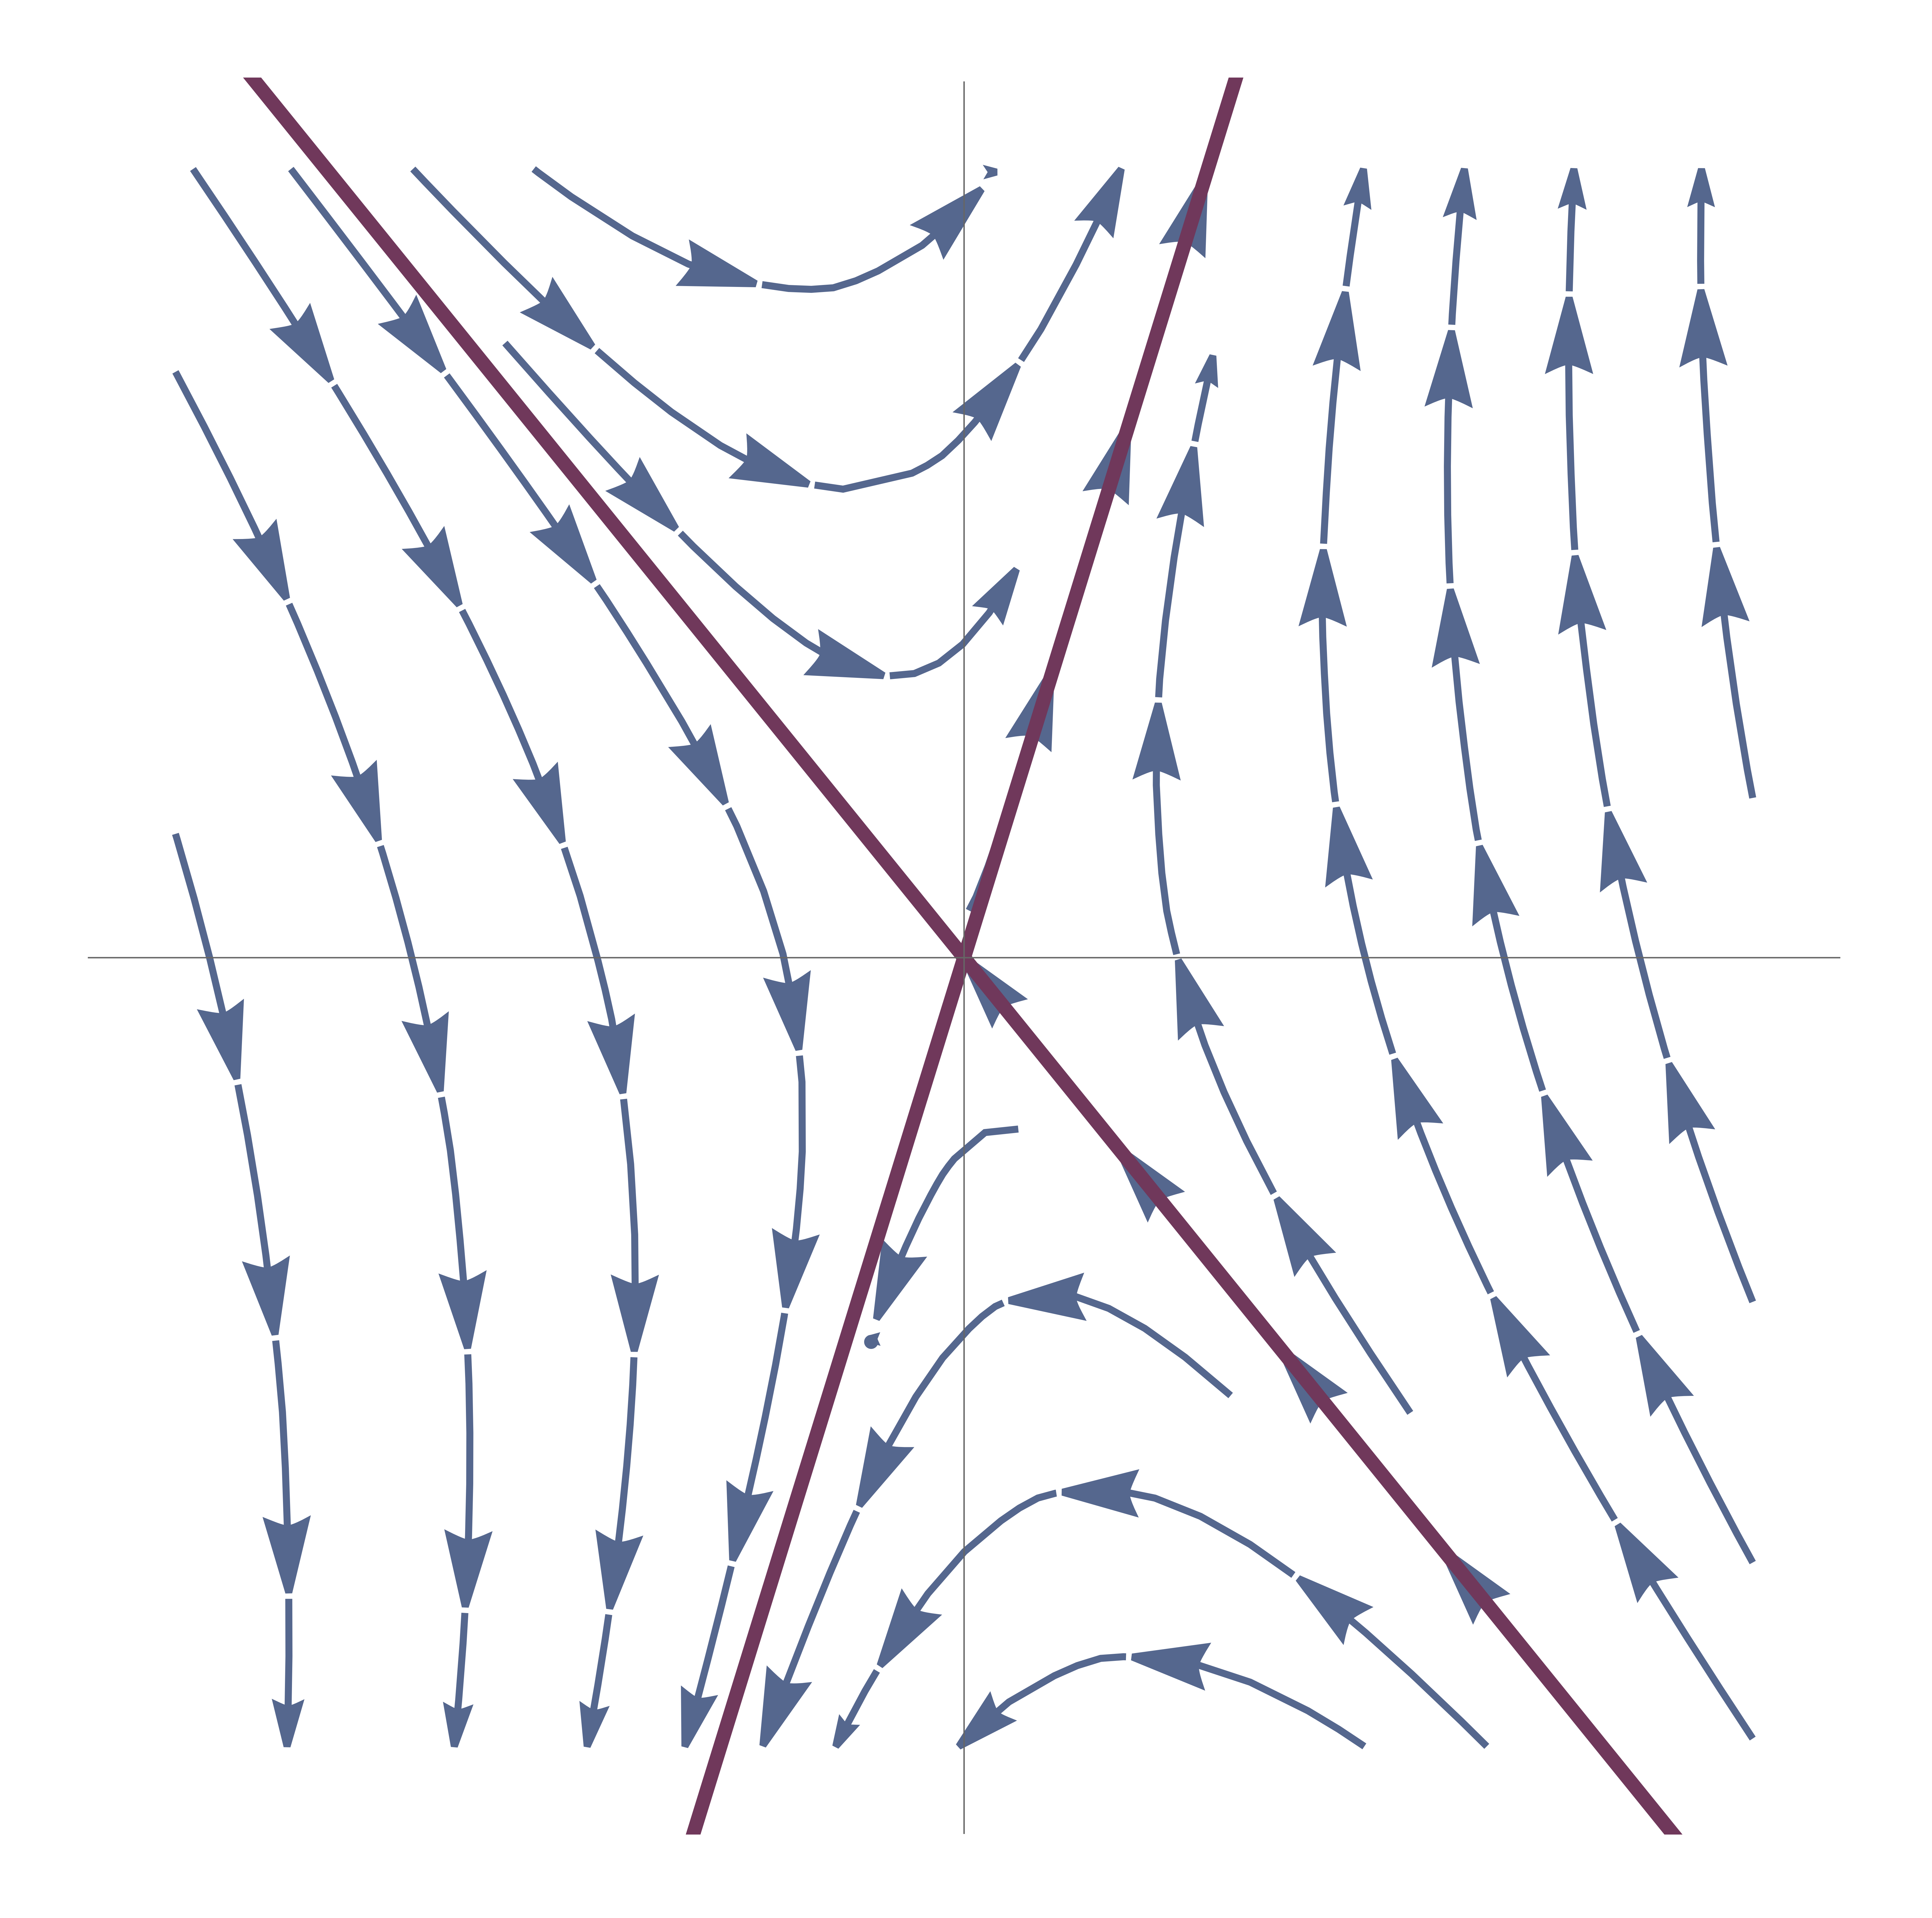
\includegraphics[width=0.4\textwidth]{fase_1}
                
                \end{example}
                
                \begin{example}
                
                    \begin{equation*}
                      x^\prime = Ax = \begin{bmatrix}
                                     -3 & \sqrt{2}\\
                                     \sqrt{2}& -2
                                     \end{bmatrix} x 
                    \end{equation*}
                    
                    Para este problema, os autovalores são $A$ são $\lambda_1 = -1$ e $\lambda_2 = -4$ e os autovetores associados são 
                $$r^{(1)} = \begin{bmatrix} \frac{1}{\sqrt{2}}\\ 1 \end{bmatrix}$$ e  $$r^{(2)} = \begin{bmatrix} -\sqrt{2}\\ 1 \end{bmatrix}.$$
                
                    A solução geral fica
                    
                    \begin{equation*}
                        x(t) = c_1 x^{(1)}(t) + c_2 x^{(2)}(t) = c_1 \begin{bmatrix} \frac{1}{\sqrt{2}}\\ 1 \end{bmatrix}e^{-t} + c_2 \begin{bmatrix} -\sqrt{2}\\ 1\end{bmatrix}e^{-4t}.
                    \end{equation*}
                    
                    Como $r^{(1)}$ será dominante para $t$ suficientemente grande (exceto se $c_1=0$), teremos soluções tangentes à reta $x_1=\sqrt{2}x_2$. As trajetórias se aproximam da origem e temos um nó localizado nesse ponto. Essa característica é comum em autovalores negativos. Se os autovalores fossem todos positivos, então o nó seria assintoticamente instável. 
                    
                    \includegraphics[width=0.4\textwidth]{fase_2}
                
                \end{example}
                
        \subsection{Autovalores Complexos}
        
            No problema $x^\prime = Ax$, quando $A$ é não-simétrica (não autoadjunta), \underline{podemos ter}  autovalores complexos. Se $A$ é real, então os autovalores devem aparecer em pares conjugados, exemplo: se $\lambda_1 = \nu + \mu i$, teremos $\lambda_1 = \nu - \mu i$. Como ficam os autovetores para essas situações? O exemplo a seguir elucidará essa questão.
            
            \begin{example}
            
                \begin{equation*}
                      x^\prime = Ax = \begin{bmatrix}
                                     -\frac{1}{2} & 1\\
                                     -1& -\frac{1}{2}
                                     \end{bmatrix} x 
                    \end{equation*}    
                
                 Os autovalores de $A$ são $\lambda_1 = -\frac{1}{2}+i$ e $\lambda_2 = -\frac{1}{2}-i$ e os autovetores associados são 
                $$r^{(1)} = \begin{bmatrix} \frac{\sqrt{2}}{2}\\ \frac{\sqrt{2}}{2}i \end{bmatrix}$$ e  $$r^{(2)} = \begin{bmatrix} \frac{\sqrt{2}}{2}\\ -\frac{\sqrt{2}}{2}i \end{bmatrix}.$$ 
                
                Finalmente temos:
                
                \begin{equation*}
                    \begin{split}
                        x(t) &= c_1 x^{(1)}(t) + c_2 x^{(2)}(t)  \\
                        &=c_1 \begin{bmatrix} \frac{\sqrt{2}}{2}\\ \frac{\sqrt{2}}{2}i \end{bmatrix}e^{(-\frac{1}{2}+i)t} + c_2 \begin{bmatrix} \frac{\sqrt{2}}{2}\\ -\frac{\sqrt{2}}{2}i \end{bmatrix} e^{(-\frac{1}{2}-i)t}.    
                    \end{split}
                  \end{equation*}
                
                O teorema a seguir nos auxiliará na busca por soluções reais para o problema.
                
                \begin{theorem}
                    Se o sistema $x^\prime = Ax$ com $A \in \mathbb{R}^{n \times n}$ tiver como solução $x(t) = u(t)+v(t)i$, então a parte real $u(t)$ e parte imaginária $v(t)$ são também soluções para o sistema.
                \end{theorem}
                
                Utilizaremos a relação de Euler - $e^{i\theta}= \cos{\theta} + i\sin{\theta}$ - para reescrever o $x^{(1)}$ que compõe a solução.
                
                \begin{equation*}
                    \begin{split}
                        x^{(1)} &= \begin{bmatrix} \frac{\sqrt{2}}{2} \\ \frac{\sqrt{2}}{2}i \end{bmatrix} e^{(-\frac{1}{2}+i)t} \\
                        &= \begin{bmatrix} \frac{\sqrt{2}}{2} \\ \frac{\sqrt{2}}{2}i \end{bmatrix} e^{(-\frac{1}{2})t}(\cos{t}+i\sin{t}) \\
                        & = \begin{bmatrix} \frac{\sqrt{2}}{2}e^{(-\frac{t}{2})}\cos{t} \\ \frac{-\sqrt{2}}{2}e^{(-\frac{t}{2})}\sin{t} \end{bmatrix} + i \begin{bmatrix} \frac{\sqrt{2}}{2}e^{(-\frac{t}{2})}\sin{t} \\ \frac{\sqrt{2}}{2}e^{(-\frac{t}{2})}\cos{t} \end{bmatrix} \\
                        x^{(1)} &= u(t) +iv(t)
                    \end{split}
                \end{equation*}
                
                Pelo teorema (1.1), $u(t)$ e $v(t)$ são soluções do sistema homogêneo. De fato, pelo Wronskiano:
                
                \begin{equation*}
                    \begin{split}
                        \mathbb{W}(u(t), v(t)) &= \begin{bmatrix} \frac{\sqrt{2}}{2}e^{(-\frac{t}{2})}\cos{t} & \frac{\sqrt{2}}{2}e^{(-\frac{t}{2})}\sin{t} \\ -\frac{\sqrt{2}}{2}e^{(-\frac{t}{2})}\sin{t}& \frac{\sqrt{2}}{2}e^{(-\frac{t}{2})}\cos{t}\end{bmatrix} \\
                        &= \frac{2}{4}(e^{-t}(\cos{t})^2 + e^{-t}(\sin{t})^2) \neq 0 \; \forall t.    
                    \end{split}
                \end{equation*}
                
                O espaço de fases para este caso está representado a seguir:
                
                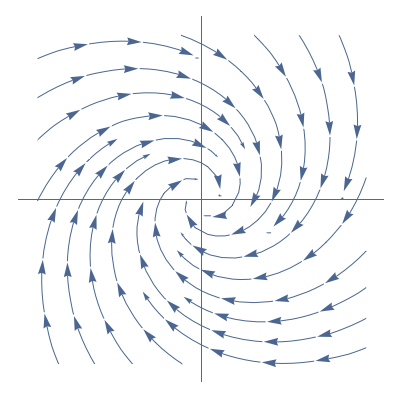
\includegraphics[width=0.4\textwidth]{fase_3}
                
                Todas as trajetórias se aproximam da origem quando $t\rightarrow \infty$, isso se deve à presença do termo $e^{-\frac{t}{2}}$. Esse espaço de fases é típico de problemas com autovalores complexos com parte real negativa. A origem é um ponto espiral e é assintoticamente estável. Para problemas com autovalores complexos e parte real positiva, o comportamento é o inverso: curvas de trajetórias que se afastam da origem (ver figura). Como ficariam as curvas de trajetórias no espaço de fases se os autovalores fossem puramente imaginários?
                
               
                
                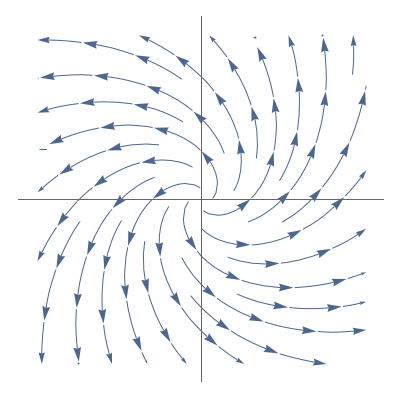
\includegraphics[width=0.4\textwidth]{fase_4}
                
                 A solução no tempo está mostrada a seguir:
                 
                 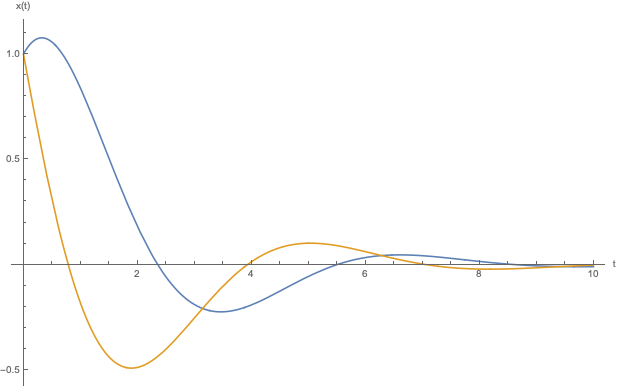
\includegraphics[width=0.45\textwidth]{tempo_1}
                
            \end{example}
            
        \columnbreak    
            
        \subsection{Autovalores Repetidos}
        
        
            O caso em que podemos ter a matriz $A$ do sistema de equações diferenciais ordinárias com autovalores repetidos será explicado através de um exemplo.
            
            \begin{example}
                \begin{equation*}
                      x^\prime = Ax = \begin{bmatrix}
                                     1 & -1\\
                                     1& 3
                                     \end{bmatrix} x 
                \end{equation*}
                
                Essa problema tem autovalor $\lambda = 2$ com multiplicidade algébrica igual a dois ($ma(\lambda = 2)= 2$). A multiplicidade geométrica é igual a um ($mg(\lambda = 2) = 1$). A multiplicidade geométrica diz quantos autovetores LI estão associados ao autovalor repetido. No caso, temos como autovetor $$r^{(1)} = \begin{bmatrix} -1 \\ 1 \end{bmatrix}.$$ Logo, temos $$x^{(1)}(t) = \begin{bmatrix} -1\\ 1 \end{bmatrix}e^{2t}.$$
                
                Por analogia ao caso de EDOs de segunda ordem com raízes da
                equação característica iguais, vamos testar se $x^{*} = \xi
                te^{2t}$ pode ser uma solução para o problema. Substituindo
                $x^{*}$ em $x^\prime = Ax$ temos
                
                \begin{equation*}
                    \begin{split}
                        (\xi te^{2t})^\prime &= A\xi te^{2t} \\
                         \xi e^{2t} + 2\xi te^{2t} &= A\xi te^{2t} \\
                         \xi e^{2t} + 2\xi te^{2t} - A\xi te^{2t} &= 0 \;(*)
                    \end{split}
                \end{equation*}
                
                Para que $(*)$ seja satisfeita para qualquer valor de $t$, é preciso que $\xi=0$. Em outras palavras, não existe solução não trivial na forma $x^{*} = \xi te^{2t}$. Como a equação $(*)$ contém termos $te^{2t}$ e $e^{2t}$, a segunda solução que procuramos deve ter a forma: $x^{*} = \xi te^{2t} + \eta e^{2t}$. Novamente substituindo em $x^\prime = Ax$:
                
                
                \begin{equation*}
                    2\xi t e^{2t} + (\xi + 2\eta)e^{2t} = A(\xi t + \eta) e^{2t}. 
                \end{equation*}
                
                Temos agora 2 equações distintas: uma ligada ao termo $t e^{2t}$ e a outra à $e^{2t}$.
                
                \begin{enumerate}[label=(\roman*)]
                    \item $2 \xi t e^{2t} = A\xi t e^{2t} \therefore (A-2I)\xi e^{2t} = 0 \therefore (A-2I)\xi = 0$ 
                    \item $2\xi e^{2t} + 2\eta e^{2t} = A \eta e^{2t} \therefore (A-2I) \eta e^{2t} = \xi e^{2t} \therefore (A-2I)\eta = \xi$
                \end{enumerate}
                
                A equação (i) já foi resolvida. A equação (ii) implica que:
                
                \begin{equation*}
                    \begin{split}
                        \begin{bmatrix}
                                     -1 & -1\\
                                     1& 1
                        \end{bmatrix} \begin{bmatrix} \eta_1 \\ \eta_2 \end{bmatrix} &= \begin{bmatrix} -1 \\ 1 \end{bmatrix} \therefore \\
                        \eta_1 + \eta_2 &= 1,
                    \end{split}
                \end{equation*}
                se $\eta_1 = -k$ ($k$ arbitrário), então $\eta_2  = 1 +k$, ou
                
                \begin{equation*}
                    \eta = \begin{bmatrix} -k \\ 1 + k \end{bmatrix} = \begin{bmatrix} 0 \\ 1 \end{bmatrix} + k \begin{bmatrix} -1 \\ 1 \end{bmatrix}
                \end{equation*}
                
                Dessa forma, conhecemos $$x^{(2)} = \begin{bmatrix} -1 \\ 1 \end{bmatrix}te^{2t}  + \begin{bmatrix}0 \\ 1  \end{bmatrix}e^{2t}$$ (a última parcela foi ignorada pois é múltipla de $x^{(1)}$). O Wronskiano de $x^{(1)}$ e $x^{(2)}$ é $\neq 0$ (verifique!). A solução geral do problema é:
                
                \begin{equation*}
                    x(t) = c_1 x^{(1)}(t) + c_2 x^{(2)}(t) = c1 \begin{bmatrix} -1 \\ 1 \end{bmatrix}e^{2t} + c_2 (\begin{bmatrix} -1 \\1 \end{bmatrix}te^{2t}
+ \begin{bmatrix} 0 \\ 1 \end{bmatrix}e^{2t})
                \end{equation*}
                
            \end{example}
            
    \section{Matrizes Diagonalizáveis e Forma de Jordan}
    
        Quando estudamos o problema de autovalor, vimos que os \underline{autovalores distintos} de um operador linear têm autovetores associados que sâo LI (teorema 4.7). O teorema a seguir apresenta um resultado derivado da linear independência dos autovetores.
        
        \begin{theorem} 
            Se $A$ é uma matriz quadrada de ordem $n$ com todos os autovetores LI, então
            
            \begin{equation*}
                T^{-1}AT=D,
            \end{equation*}
            onde $T$ é uma matriz cujas colunas são formadas pelos autovetores de $A$ e $D$ é uma matriz $n \times n$ diagonal, diagonal esta formada pelos autovalores de $A$.
        \end{theorem}
        
        \begin{corollary}
            Caso particular: Se $A$ for uma matriz simétrica de ordem $n$ com todos os seus autovalores distintos, então $T$ é uma matriz ortogonal se as suas colunas forem formadas pelos \underline{autovetores normalizados} de $A$. Como $T$ é ortogonal, vale a relação:
            
            \begin{equation*}
                T^{T}T=TT^{T}=I,
            \end{equation*}
            ou seja, $T^{-1} = T^{T}$, logo 
            \begin{equation*}
                T^{T}AT=D,
            \end{equation*}
            onde  $D$ é uma matriz $n \times n$ diagonal, diagonal esta formada pelos autovalores de $A$.
        \end{corollary}
        
        \begin{example}
            Aplicação de matrizes diagonalizáveis para a resolução de ODEs homogêneas: vamos resolver o Exemplo 1.1 utilizando a propriedade vista no Teorema 2.1.
            
            
            \begin{equation*}
                x^\prime = Ax = \begin{bmatrix}
                                     1 & 1\\
                                     4 & 1
                                     \end{bmatrix} x 
            \end{equation*}
            
        \end{example}
        
    \section{Sistemas de EDOs Lineares Não-Homogêneas}
    
        Os sistemas de EDOs lineares não-homogêneas são sistemas na forma:
        
        \begin{equation*}
                x^\prime (t) = Ax(t) + f(t)
            \end{equation*}
        onde $A$ é uma matriz quadrada formada por coeficientes constantes de ordem $n \times n$ e $$ x^\prime (t) = \begin{bmatrix}
x_1^\prime\\
x_2^\prime\\
\vdots\\
x_n^\prime
\end{bmatrix},$$ $$ x(t) = \begin{bmatrix}
x_1 \\
x_2 \\
\vdots\\
x_n 
\end{bmatrix}$$ e $$ f(t) = \begin{bmatrix}
f_1 (t) \\
f_2 (t) \\
\vdots\\
f_n (t) 
\end{bmatrix}.$$

        \subsection{Método da Diagonalização da Matriz}
        
        Se a matriz $A$ tiver autovalores distintos,  podemos diagonalizá-la 
        
        \begin{equation*}
            T^{-1}AT=D,
        \end{equation*}
        lembrando que se $A=A^T$, temos $T^{-1} = T^T$. Utilizaremos essa propriedade de diagonalização para reescrever o sistema $x^\prime = Ax + f(t)$ fazendo a seguinte mudança de variáveis:
        
        $$x = Ty \therefore x^\prime = Ty^\prime.$$
        
        A equação transformada fica:
        
        $$y^\prime = Dy + T^{-1}f(t).$$ Como $D$ é diagonal, as equações ficam desacopladas e peidemos utilizar a técnica de fatores integrantes para resolvê-las. O exemplo a seguir mostrará como funciona.
        
        \begin{example}
            \begin{equation*}
                x^\prime = \begin{bmatrix}
                                     -2 & 1\\
                                     1 & -2
                                     \end{bmatrix} x + \begin{bmatrix} 2e^{-t} \\ 3t\end{bmatrix}.
            \end{equation*}    
        \end{example}
        
        \subsection{Forma de Jordan e Autovalores Repetidos para Sistemas de EDOs}
        
            A decomposição $T^{-1}AT$ só será diagonal se os autovalores forem distintos. Quando os autovalores tem multiplicidade algébrica maior que um, a decomposição $T^{-1}AT$ pode resultar numa forma de Jordan composta por blocos que dependerão da multiplicidade geométrica.
            
            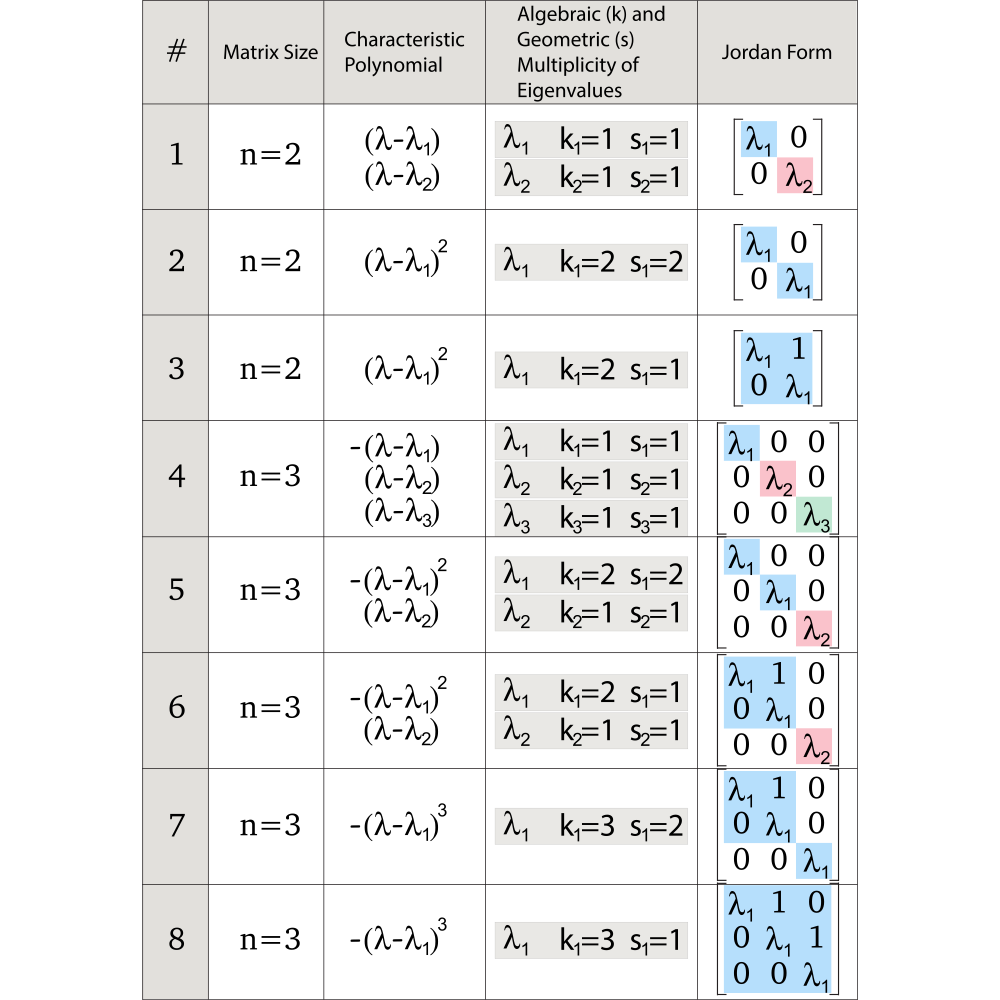
\includegraphics[width=0.5\textwidth]{jordan-matrices.svg}
            
            O exemplo a seguir esclarecerá a questão sobre as formas de Jordan.
        
            \begin{example}
                \begin{equation*}
                    x^\prime = \begin{bmatrix}
                                         3 & 1 &1\\
                                     2 & 2 & 1\\
                                    -4 & -3 & -2
                                     \end{bmatrix} x + \begin{bmatrix} 1 \\ e^{t} \\ e^{2t} \end{bmatrix}.
                \end{equation*}     
            \end{example}
            
        \subsection{Resolução por Matrizes Fundamentais}
        
            \subsubsection{Matriz Fundamental}

            \begin{definition}
                Matriz fundamental: Sejam $x^{(1)}(t),x^{(2)}(t), \ldots,
                x^{(n)}(t)$ um conjunto de $n$ soluções LI de $x^\prime = Ax$. Definiremos como matriz fundamental a matriz $\Phi (t)$ dada por:
                
                \begin{equation*}
                    \Phi (t) = \begin{bmatrix}  x^{(1)}(t) & x^{(2)}(t)& \ldots& x^{(n)}(t) \end{bmatrix}
                \end{equation*}
                
                A matriz $\Phi (t)$ atende ao problema $\Phi^\prime = A \Phi$.
                
            \end{definition}
            
            Com $\Phi (t)$ podemos resolver o problema de valor inicial $x^\prime =  Ax$, com $x(t_0)=x_0$. A solução geral de $x^\prime = Ax$ é
            
            $$x = \Phi C,$$ onde $C$ é um vetor de constantes. Aplicando as condições iniciais $x(t_0)=x_0$, temos
            
            $$x_0 = x(t_0) = \Phi (t_0)C$$, por sua vez, o vetor $C$ fica determinado através de:
            
            $$C=\Phi^{-1} (t_0)x_0.$$
            
            \begin{example}
                \begin{equation*}
                    x^\prime = \begin{bmatrix}
                                         5 & 3 \\
                                     -6 & -4\\
                                     \end{bmatrix} x. 
                \end{equation*}     
            Como condições iniciais
            
            $$x(0) = \begin{bmatrix} 1 \\ 2 \end{bmatrix}.$$
            
            \end{example}
            
            \subsubsection{Problemas Não-Homogêneos e Matrizes Fundamentais}
            
            Retomando a forma mais geral de um sistema de EDOs Lineares:
            
            $$x^\prime(t) = Ax + f(t),$$ utilizaremos o conceito de matriz fundamental para encontrar soluções gerais na forma
            
            $$x(t) = \Phi (t)C + x_p (t),$$ de maneira que 
            
            $$x^\prime_p = Ax_p + f(t).$$
            
            Vamos assumir que $x_p = \Phi (t)c(t)$. Derivando essa igualdade em relação ao tempo temos
            
            $$x^\prime _p = \Phi^\prime c + \Phi c^\prime = A\Phi c + \Phi c^\prime,$$ ou
            
            $$x^\prime _p  - Ax_p = \Phi c^\prime.$$ Notemos que $x^\prime _p  - Ax_p = f$, isso implica que
            
            $$\Phi c^\prime = f \therefore c^\prime = \Phi^{-1}f.$$ Agora basta integrarmos essa expressâo e conheceremos a solução particular $x_p (t)$:
            
            $$x_p (t) = \Phi (t) \int^{t}\Phi^{-1}(s)f(s)ds.$$ A solução geral para o problema nâo-homogêneo pode ser encontrado por
            
            $$x(t) = \Phi (t)C + \Phi (t) \int^{t}\Phi^{-1}(s)f(s)ds.$$ Com as condições iniciais, temos a solução particular
            
            $$x(t) = \Phi (t)\Phi^{-1}(t_0)x_0 + \Phi (t) \int^{t}_{t_0}\Phi^{-1}(s)f(s)ds.$$
            
            \begin{example}
                Resolver a EDO de segunda ordem $x^\prime^\prime + x = 2
                \cos{t}$, com $x(0)=4$ e $x^\prime (0)=0$.
            \end{example}
            
            

\end{multicols*}

\end{document}
